\addcontentsline{toc}{section}{Signal Flow in Neural Networks}
\section*{Signal Flow in Neural Networks}

A Feedforward Fully Connected Neural Network (FCNN) is a Neural Network architecture where each neuron in one layer is connected to every neuron in the subsequent layer.

\begin{figure}[h]
    \centering
    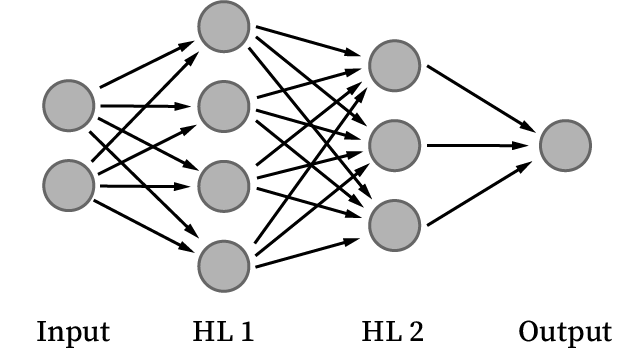
\includegraphics[width=0.75\linewidth]{Images/fcnn.png}
    \caption{A Feedforward Fully Connected Neural Network (FCNN).}
    \label{fig:fcnn}
\end{figure}

A FCNN learns by iteratively performing two main steps: the forward pass and the backward pass.

\paragraph{Forward pass} The input data is propagated through the network, layer by layer, to produce an output prediction. This prediction is then compared to the true target values using a loss function, which quantifies the prediction error.

\paragraph{Backward pass} The network uses the computed loss to adjust its internal parameters. This is done by propagating the error backward through the network and updating the weights to minimize the loss. The process of forward and backward passes is repeated for multiple iterations, gradually improving the model's performance.

This step is the heart of the learning process, as it allows the network to learn from its mistakes and improve its predictions over time.
